\documentclass[../../main.tex]{subfiles}

 \lhead{User Testing}
 
\begin{document}

\section{User Testing}
	Once the implementation of the system to allow the user to move themselves around a virtual space had been completed, the plausibility of the methods used were tested. The following sections present the aims of the user tests in full, the procedure required to fulfil the set objectives followed by the results and a discussion.

	In total, seven students took part in the user tests, all of which were studying audio related subjects.

	\subsection{User Testing Aims}
		There were a total of 3 user tests, with the third being split into two parts with an identical procedure. The aims of each test were as follows:

		\textbf{Test \#1:} Investigate the effect of using the synthetic \ac{RIR}'s as opposed to the previously used real \ac{RIR}'s used.

		\textbf{Test \#2:} Investigate how far the user has to be moved before they notice that they have been moved using synthetic \ac{RIR}'s

		\textbf{Test \#3.1:} Investigate which \ac{RIR} grid provides the user with the best sense of mobility

		\textbf{Test \#3.2:}  Investigate whether the users opinion changes when using a position feedback system

			Before the tests were conducted, each participant was presented with a `Test Participant Form', informing them of the aims of the tests and the procedures that were to follow. As they were going to be stood inside the speaker array, the answers provided by each participant were taken down on their behalf. At the end of the experiment the answers were checked and signed by the participant assuring that their answers had been taken down accurately. The form provided to the participants can be found in~\nameref{appendixD}.

			Before each test, the participants were allowed two `dummy runs', allowing them to get used to the system without having their answers recorded, with the intention of removing the disadvantage of being unfamiliar with the system for the first few questions of each test. They were also informed that during each test they were allowed to turn their head in the space to obtain a more natural listening experience.

	\subsection{Statement of Hypothesis}

	\subsection{Test \#1}
	

		\subsubsection{Procedure}

			To investigate the difference in the perception of distance moved when using either synthetic or real \ac{RIR}'s, the following procedure was carried out:

			%The user was placed at position (1) (using a real \ac{RIR}, in the centre of the virtual space and asked to say the word `Bob'. The were then moved to a new position and asked to repeat themselves. THen, using the \ac{RIR}'s produced in Odeon the were asked to do the same again. They were then asked whether 

			The participant was told that two methods were going to be investigated during this test, method \textbf{A} and method \textbf{B}. The participant was not told that in method \textbf{A}, the real \ac{RIR} measurements from Hendrix Hall were going to be used to move them around the room and in method \textbf{B} the synthetic \ac{RIR}'s produced in Odeon were going to be used. The participant was told that using method \textbf{A}, they were going to be placed somewhere in the virtual space and that they would be asked to say the word `Bob'. They would then be moved to another position in the space and asked to repeat themselves. This procedure would the be repeated, however this time using method \textbf{B}. They were then asked to state whether they felt they had:

			\begin{center}
			    \begin{tabular}{l}
			       1) Moved a \textbf{shorter} distance than they had in \textbf{A}\\
			       2) Moved the \textbf{same} distance they had in \textbf{A}\\
			       3) Moved a \textbf{further} distance than they had in \textbf{A}\\
			       4) I don't know\\
			    \end{tabular}
			\end{center}

			This was repeated three times where the distances used for mathes A and B were kept the same. For the final two trials, the distances between the two methods were changed. The left of figure~\ref{test1} shows an illustration of the virtual space indicating where the four \ac{RIR} locations used for the test are. The black numbers indicate the coordinates of the \ac{RIR}'s  relative to the top left corner of the room (note that the x and y axis are opposite to convention due to the way the building was modelled in Google SketchUp), and the red numbers are used to indicate which location the user was moved to during each test, shown on the right in figure~\ref{test1}.



			%-------------Test 1 Image and Table-------------%
			\begin{figure}[H]
				\begin{minipage}{0.5\textwidth}
					\begin{figure}[H]
						\centerline{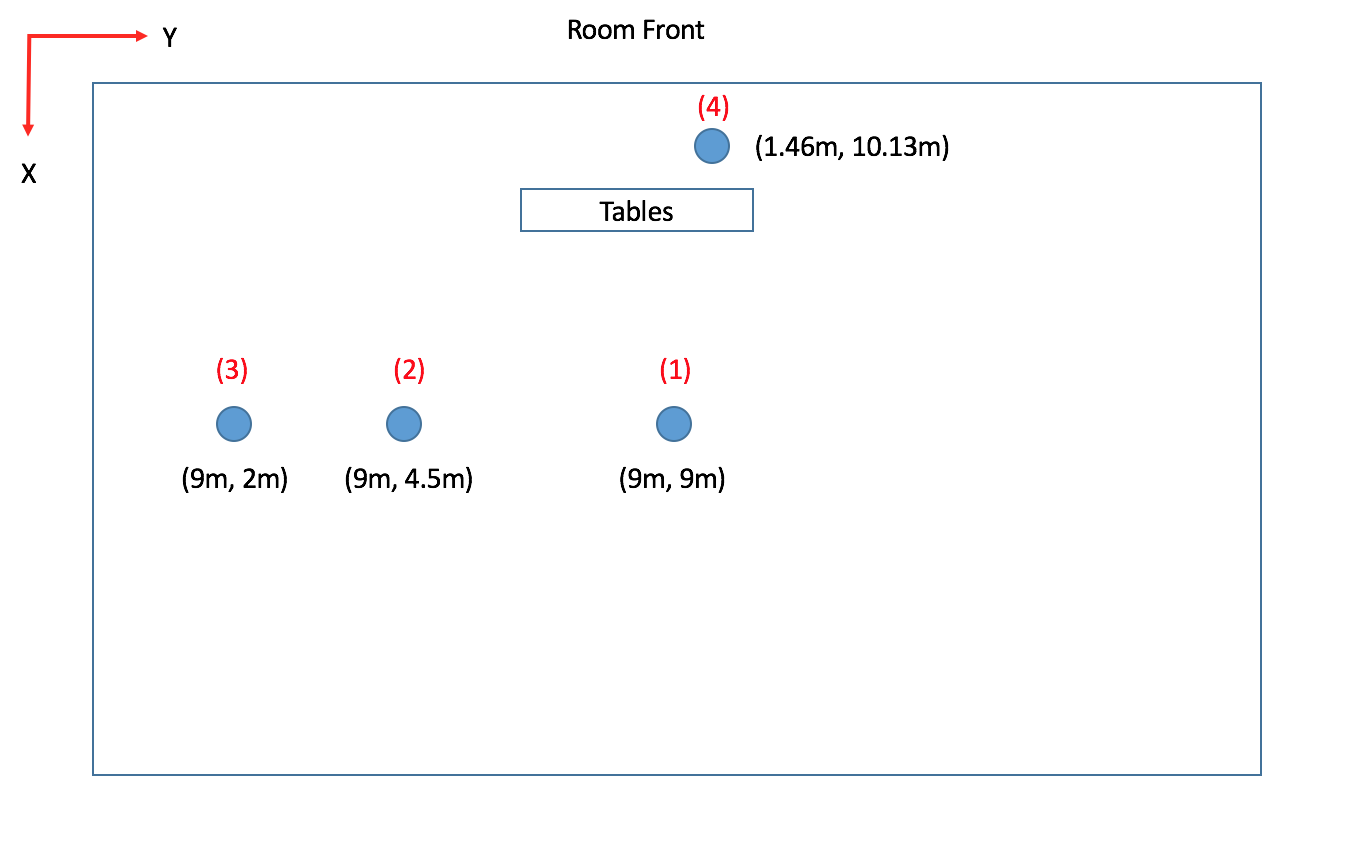
\includegraphics[scale = 0.5]{Sections/userTesting/images/test1/roomPositions3.png}}
					\end{figure}			
				\end{minipage}
				~
				\hspace{25mm}\begin{minipage}{0.5\textwidth}
				\begin{table}[H]
				    \begin{tabular}{|c|cc|cc|} \hline
				        \multirow{2}{*}{Trail} & \multicolumn{2}{c|}{Real RIR \textbf{(A)}} & \multicolumn{2}{c|}{Odeon RIR \textbf{(B)}}\\ \cline{2-5}
				            & Start & End & Start & End \\ \hline
				          1 & (1) & (2) & (1) & (2)\\
				          2 & (1) & (3) & (1) & (3)\\
				          3 & (1) & (4) & (1) & (4)\\ \hline
				          4 & (1) & (3) & (1) & (4)\\ 
				          5 & (4) & (1) & (1) & (3)\\ \hline
				    \end{tabular}
				\end{table}
				\end{minipage}
				\caption{\textbf{Left:} Illustration of the \ac{RIR} locations used in user test \#1. \textbf{Right:} Table showing the pairs of positions the participant was moved to, corresponding to the positions shown in the diagram on the left.}
				\label{test1}
			\end{figure}

		\subsubsection{Results}
			The participants answers for user test \#1 were taken and averaged across all five trials. Figure~\ref{test1Results} shows these results, showing the percentage of correct and incorrect answers given (left) and the percentage of each type of answer given (right). It can be seen that only 23\% of the answers given across all trials and participants were correct, indicating there being difficult comparing the two distances moved.

			%-------------Pie 1-------------%
			\begin{figure}[H]
				\begin{subfigure}{0.5\textwidth}
					\centerline{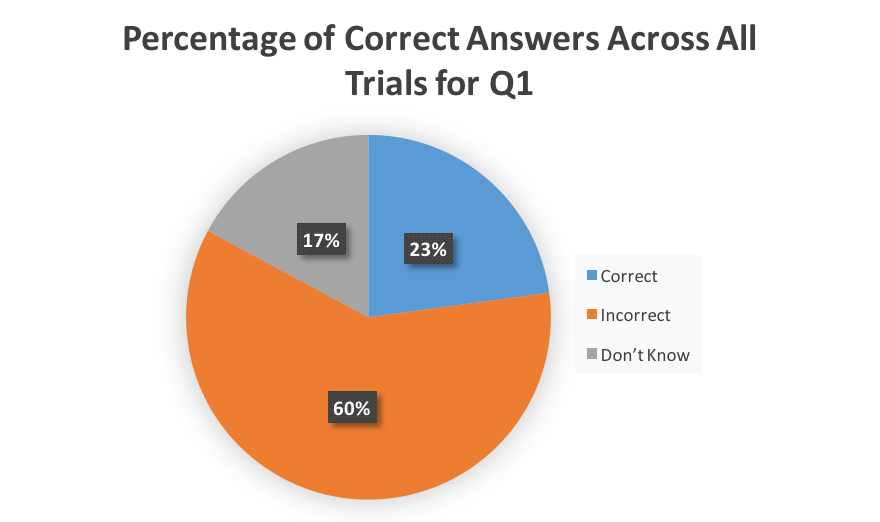
\includegraphics[scale = 0.7]{Sections/userTesting/images/test1/Q1Pie1_edit.png}}
				\end{subfigure}
				~
				\begin{subfigure}{0.5\textwidth}
					\centerline{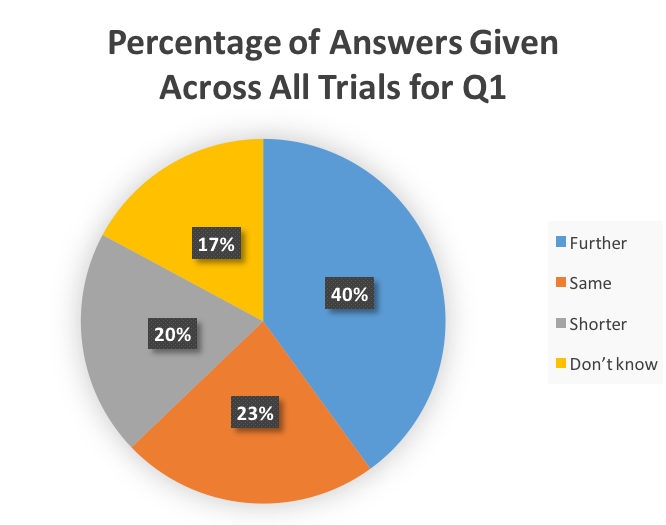
\includegraphics[scale = 0.7]{Sections/userTesting/images/test1/Q1Pie2.png}}
				\end{subfigure}
				\caption{Pie charts showing the results of user test \#1}
				\label{test1Results}
			\end{figure}


			The pie chart on the right shows that more commonly, people thought that they were moving a further distance when the synthetic \ac{RIR}'s were used. It can be seen in the table in figure~\ref{test1} that the expected answers are as follows:

			\begin{center}
			\begin{tabular}{c l}
			\textbf{Trial} & \textbf{Correct Answer} \\
			1-3 & Same \\
			4 & Shorter \\
			5 & Further
			\end{tabular}
			\end{center}

			However, an interesting result can be seen when breaking down the answers given into their respective trials, as shown by the three pie charts in figure~\ref{Q1Trials}. When the distance moved was either the same (trials 1-3) or shorter (trial 4), more people tend to answer that they had moved further, more so when they had actually moved a shorter distance. When the distance moved was actually further, the answers are evenly split between `Further', `Same' and `Don't Know'. This negative correlation between expected answer and given answer suggests that the pie chart on the right in figure~\ref{test1Results}, showing that the majority of people thought they were moving further throughout all trials, is not influence by the fact that people got the answer to trial 5 correct, indicating that it is the use of the synthetic \ac{RIR}'s themselves that cause this perception.


			%-------------Pie 1-------------%
			\begin{figure}[H]
				\centerline{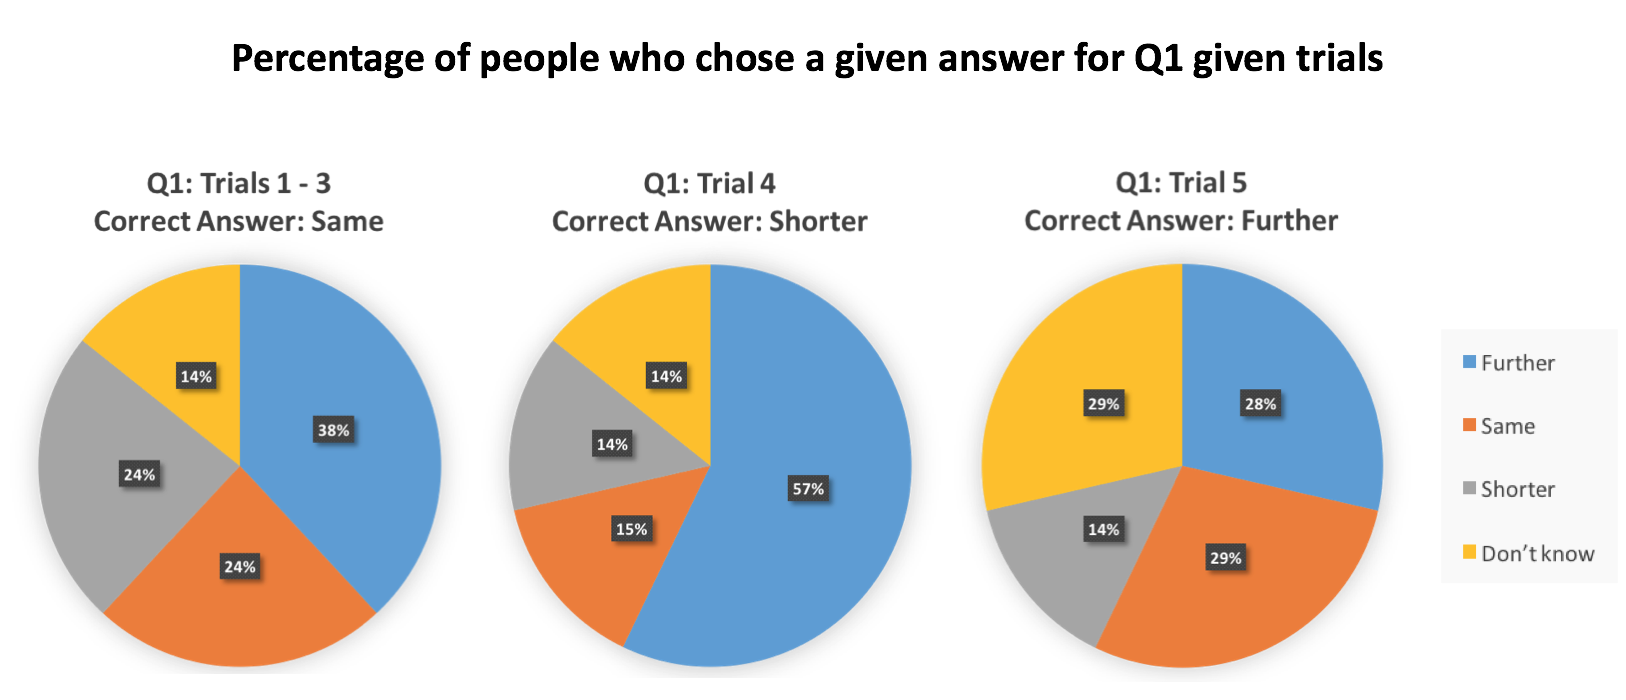
\includegraphics[scale = 0.6]{Sections/userTesting/images/test1/Q1Trials.png}}
				\caption{Three pie charts showing the percentage of answers given for: \textbf{Left:} Trials 1- 3, \textbf{Centre:} Trial 4, \textbf{Right:} Trial 5.}
				\label{Q1Trials}
			\end{figure}

		\subsubsection{Discussion}

			%Reason so little got the answer right may be because they expect to have moved. Also because the input (them saying Bob) might have been different every time.

			Due to the small percentage of correct answers given, it is apparent that comparing the difference in distance moved is not easy. For the system used, there may be 2 reasons for this:

			\begin{tabular}{l p{0.9\textwidth} }
			1) & \textbf{The test is too hard} \\
			& Asking the participants to not only compare how two different locations sound to each other, but compare that difference to how another two sound compare to each other may have been too much to remember at once. This may have led to participants guessing answers as opposed to giving an answer based on opinion, even though the `I Don't Know' option was available. \\
			2) & \textbf{Inaccurate \ac{RIR}'s} \\
			& It has been mentioned in section~\fullref{RIRtrimming} that due the fact that the \ac{RIR}'s had to be trimmed due to system latency, much needed direct wall reflections are not present for surfaces less than approximately 3.78m away, thus affecting the ability to accurately assess ones location within a space.
			\end{tabular}

		\subsection{Test \#2}

			\subsubsection{Procedure}
				The second user test is similar to that of the first test, though a little more simple. Figure~\ref{test2} shows 8 \ac{RIR} locations, where (1) is in the centre of the room. The participant was placed at position (1) and asked to say the word `Bob'. They would then be moved closer to the left wall, asked to repeat themselves and asked whether they thought they had moved or not, simply answering yes, no or `I Don't Know'. This was done 7 times, moving the participant a further distance each time. The table on the right in figure~\ref{test2} shows the start and end position for each trial.

							%-------------Test 1 Image and Table-------------%
			\begin{figure}[H]
				\begin{minipage}{0.5\textwidth}
					\begin{figure}[H]
					\hspace{0mm}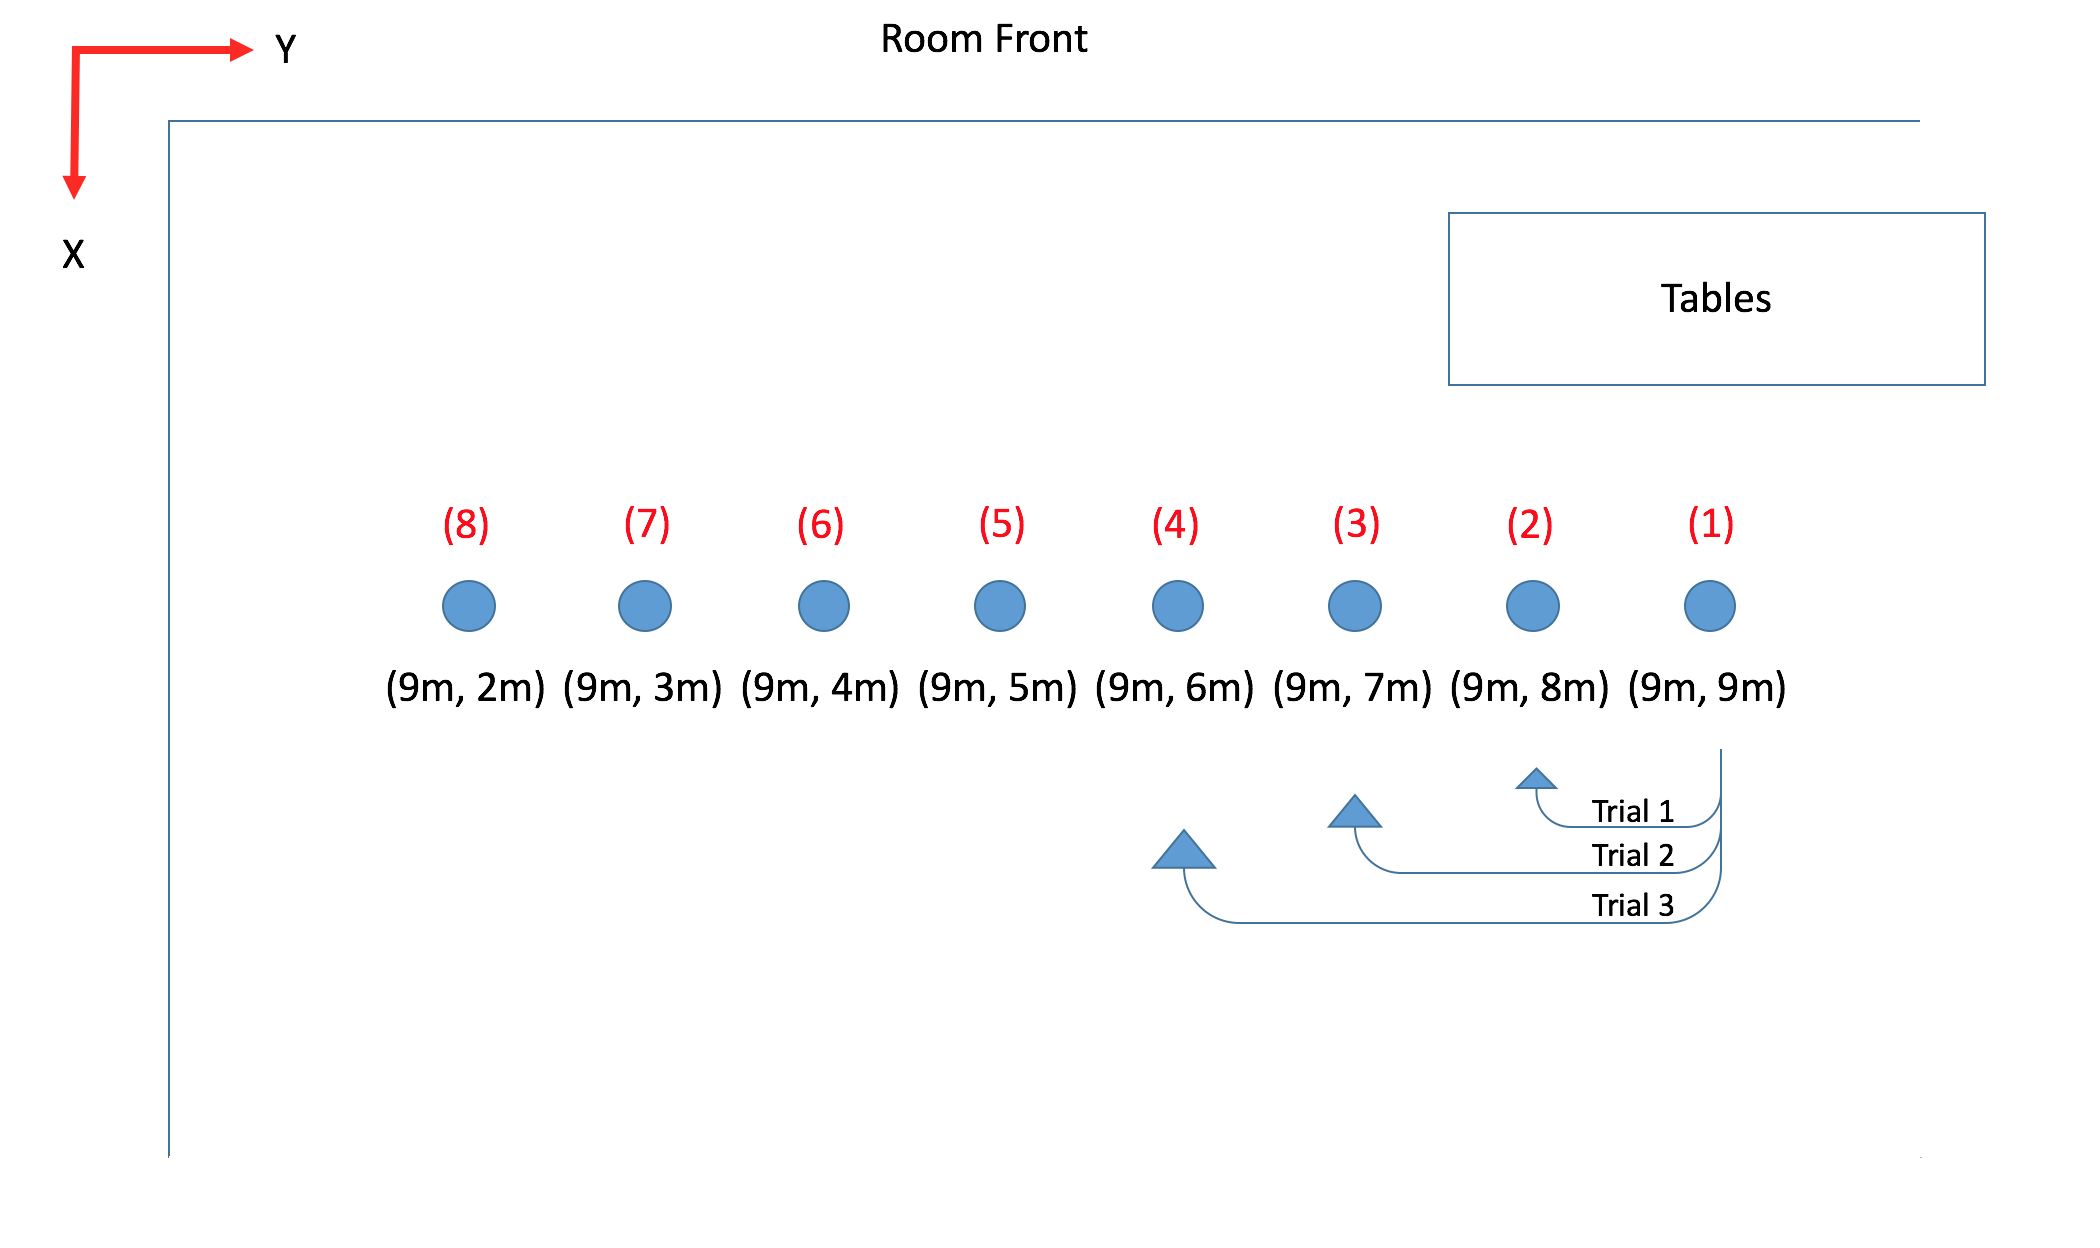
\includegraphics[scale = 0.3]{Sections/userTesting/images/test2/test2Positions2.png}
					\end{figure}			
				\end{minipage}
				~
				\begin{minipage}{0.5\textwidth}
				    \hspace{35mm}\begin{tabular}{|c|c|c|} \hline
				        \multirow{2}{*}{Trail} & \multicolumn{2}{c|}{Position (x,y)} \\ \cline{2-3}
				             & Start & End \\ \hline
				          1 & (1) & (2) \\
				          2 & (1) & (3) \\
				          3 & (1) & (4) \\
				          4 & (1) & (5) \\
				          5 & (1) & (6) \\
				          6 & (1) & (7) \\
				          7 & (1) & (8) \\ \hline
				    \end{tabular}
			    \end{minipage}
			    \caption{\textbf{Left:} Illustration of the \ac{RIR} locations used in user test \#2. \textbf{Right:} Table showing the pairs of positions the participant was moved to, corresponding to the positions shown in the diagram on the left.}
				\label{test2}
			\end{figure}

			\subsubsection{Results}

				Figure~\ref{test2results} shows a line graph of the results obtained from user test \#2, showing on how many participants answered `Yes', `No' or `Don't Know' for each of the trials.

				The original hypothesis to this test was that the participants were unlikely to notice that they had moved for the first few trials as they were being moved such a short distance (1m, 2m), with the expectation that they would notice when they were being moved much larger distances, hence the reason there were moved 1m closer to the wall in each trial. However, it was found that all participants answered `Yes' for the first trial (movement of 1m towards the left wall) and all other trials resulted in a number of participants giving an answer other than `Yes'. Instead of a positive correlation between distance moved and `Yes' answers given, there appears to be a dip from trials 2-4.

				Figure~\ref{test2rate} shows a compressed version of the data in figure~\ref{test2results}, clearly indicating that at no point during the test, do any of the participants agree whether they have definitively moved or not. This indicates that the perception of mobility may differ from person to person. This could potentially be based on their listening experience, or possibly due to consistency of the input signal (saying the word ``Bob'') being different between participants.

				%-------------Test 2 Results-------------%
				\begin{figure}[H]
					\centerline{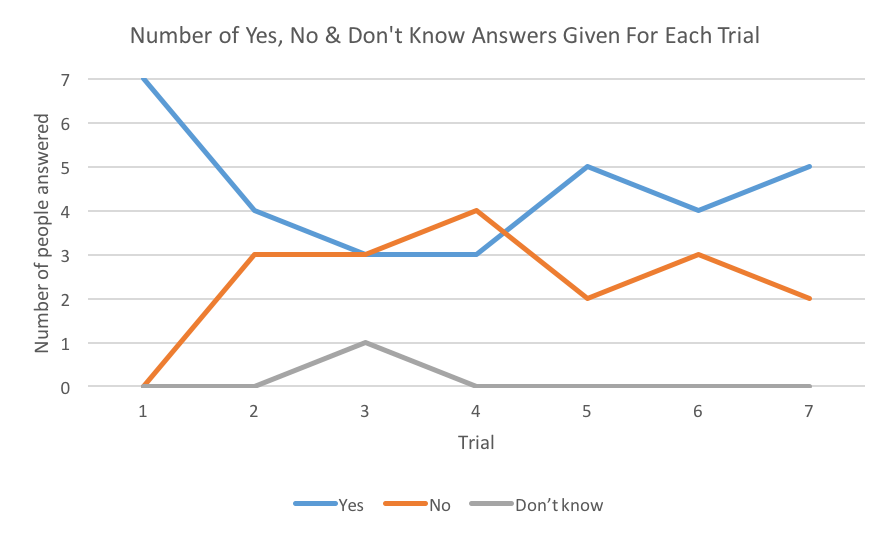
\includegraphics[scale = 1]{Sections/userTesting/images/test2/Q2_edit.png}}
					\caption{Line graph of the results from user test \#2 showing the number of participants who answered `Yes', `No' or `Don't Know' for each of the trials.}
					\label{test2results}
				\end{figure}

				%-------------Test 2 Results-------------%
				\begin{figure}[H]
					\centerline{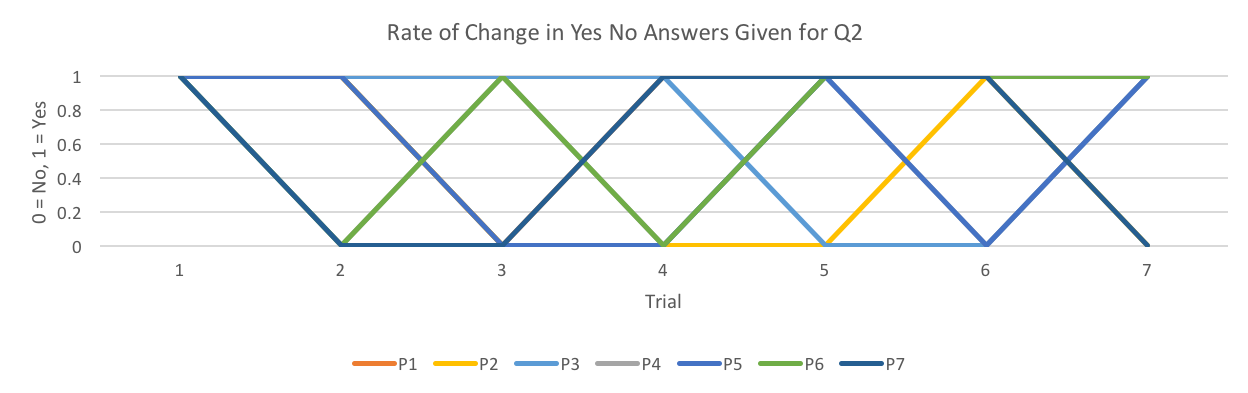
\includegraphics[scale = 0.7]{Sections/userTesting/images/test2/rateofchange.png}}
					\caption{Line graph showing the rate at which participants give `Yes' or `No' answers, showing that at no point do all participants agree whether they have definitively moved or not. (The single `Don't No' answer has been omitted here)}
					\label{test2rate}
				\end{figure}

			\subsubsection{Discussion}

				Comparing the results to the original hypothesis, excluding the first two trails, there seems to be more people noticing movement as the distance moved increases. These first two trials may have been subject to a bias, where the user is expecting to be moved. This however can not be backed up and remains a speculation. 

				 The fact that some participants could still not tell that they had moved at greater distances indicates that the differences between these \ac{RIR}'s may not be enough to convince some people that they have moved. A potential variable that may have caused some unexpected answers is the fact that no person can repeat themselves perfectly.

				Other causes for these results could be one of the following:

				\begin{tabular}{l p{0.9\textwidth}}
				1) & That the \ac{RIR}'s used do not contain enough information regarding the users location. \\
				2) & The participants answering `No' simply don't know or do not hear that they expect to hear when moving in a room.\\
				3) & The inconsistency in repeating themselves has more of an effect on their perception of location than the actually room acoustics.
				\end{tabular}


		\subsection{Test \#3}
			\label{usertests:test3}

			\subsubsection{Procedure}
				The participants were presented with an iPad and informed that it could be used to draw a path within the virtual space which they would then be moved around. Five trials were run, each using a different \ac{RIR} grid, previously explained in section~\fullref{odeon:grids} and displayed in section~ \fullref{rirlocations} in figure~\ref{bulkRIRs} (1m separation) and in \fullref{appendixB} as figures~\ref{2m},\ref{3m},\ref{4m},\ref{5m} (2m - 5m separation respectively). The following table shows which trial used with \ac{RIR} grid, stating the distance between \ac{RIR} locations and the number of \ac{RIR} locations within that grid:

				\begin{center}
					\begin{tabu} to 0.9\textwidth{X[1,c] X[2,c] X[2,c]}
					Trial & \ac{RIR} Location Separation & Number of Positions Available \\
						1 & 1m & 240 \\
						2 & 2m & 112 \\
						3 & 3m & 25 \\
						4 & 4m & 12 \\
						5 & 5m & 9 \\
					\end{tabu}
				\end{center}
				\vspace{5mm}
				In each trial, the participant was asked to draw a path and listen to an audio sample \cite{trumpet} (\textbf{[REFERENCE AUDIO SAMPLE]} which was played in place of the participant speaking/singing to provide a constant sound source (as determining movement would be difficult with inconsistent speaking). They were then asked to rate on a scale of 1-10 the quality of mobility, where 1 = extremely ``jumpy'' movement and 10 = completely smooth movement, or to give the answer `N/A' if they had difficulty telling whether they were moving or not.

				The five trials were run twice, once without a dot showing them where they are in the virtual space and once with a dot. This was to test whether their perception of how `smoothly' they were moving around the space changed when they could see exactly where they were.

			\subsubsection{Results}

				The results in figure~\ref{score} show that on average, using the grid with \ac{RIR} locations separated by 4m when the location tracking dot was not used (blue bars), scored the highest. However it only scoring an average 0.5 higher than the grid using 3m of separation. By looking at that variance of the answers given in figure~\ref{variance}, it can be seen that the grid with 3m separation was rated much more consistently that the grid with 4m separation.

				When the location tracking dot was used, it was found the using the grid with 4m separation on average scored the highest with only a slightly higher variance than the grid of 2m separation, which scored second highest.

				Participants were asked to provide comments on using the system both with and without the location tracking dot. Several participants commented on trial number 3, mentioning that it was easier to tell that they were moving than the prior trials. Comments on using the location tracking dot referred to the fact that it helped them determine what they should be listening for, one participant in particular referring to the speed the dot was moving at was important, given its variance across trials.

				%-------------Test 3 results-------------%

				\begin{figure}[H]
					\begin{subfigure}{1\textwidth}
						\centerline{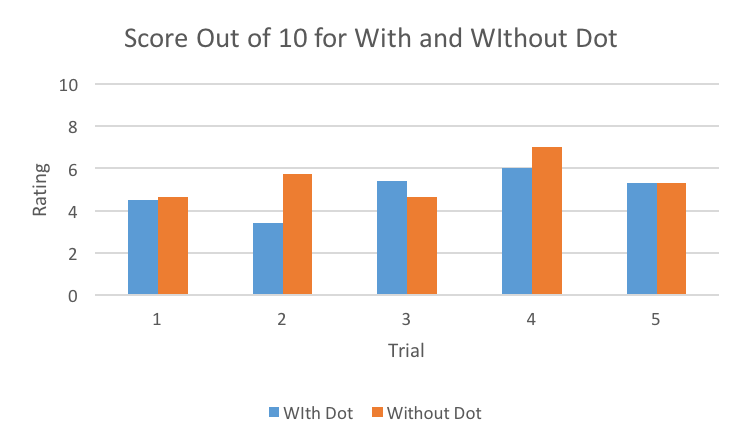
\includegraphics[scale = 0.7]{Sections/userTesting/images/test3/Q3Score.png}}
						\caption{Average score given from 1 - 10 (1 = jumpy movements, 10 = smooth movement) for each of the trials 1 - 5 (1 = 1m \ac{RIR} separation, 5 = 5m \ac{RIR} separation)}
						\label{score}
					\end{subfigure}
					
					\begin{subfigure}{1\textwidth}
						\centerline{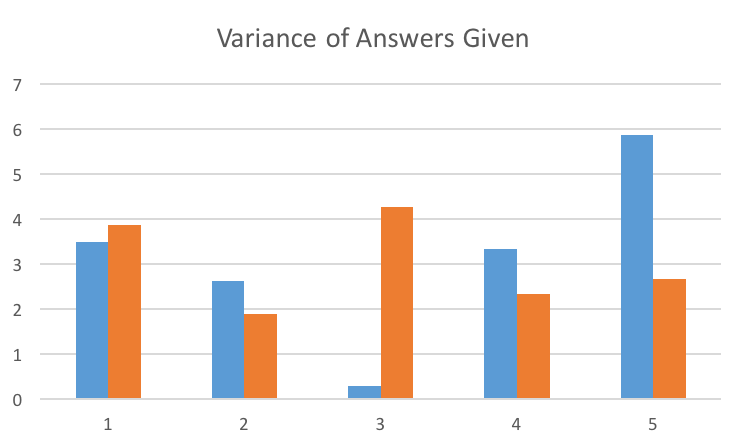
\includegraphics[scale = 0.7]{Sections/userTesting/images/test3/Q3Variance.png}}
						\caption{Variance of the answers given in figure~\ref{score}}
						\label{variance}
					\end{subfigure}
					\caption{Pie charts showing the results of user test \#1}
					\label{test1Results}
				\end{figure}



			\subsubsection{Discussion}

			%Less RIRs, move faster, not good
			As discussed in section~\fullref{iteration3}, the rate at which the user is moved from one \ac{RIR} location to another is determined by a timer which runs at a constant speed. This means that when the distance between \ac{RIR} locations is greater, the speed at which the participant is moved across the room is greater. The inconsistency in movement speed had an obvious effect on the perception of movement when using different sized \ac{RIR} grids, where participants had commented that it felt like they were moving faster. For example, it had been noted by some participants that in trials 1 (1m \ac{RIR} separation), it did not feel like they were moving. This is most likely because moving 1m every 2.5 seconds is too slow to notice. However, due to the compromise that had to be made due to system speed, they could not be moved any faster than this. This may have led to participants giving the trials that used more spacious \ac{RIR} placement a higher score (such as trial 3 and 4) as they could hear themselves moving more obviously due to the greater distance travelled, thus thinking that they were moving more smoothly.

			Due to the issues mentioned, the author concludes that these results cannot be used to confidently suggest how many \ac{RIR}'s are required to convince the user can move freely in the \ac{VAE} and are therefore inconclusive. In order to obtain results regarding the original question, either the current system should be improved to keep the speed of the user constant, or a way to implement the original system, iteration 1, should be investigated.

		\subsection{User Tests Discussion and Summary}

			\subsubsection{Test Length}
				%The test were long, therefore the questions were kept shorter than they should have been. For example, In Test 2 it would have been beneficial to run the same test multiple times to check the variance in their answers, however it was this would have taken far too long to do, especially given the tediousness of the tests.

				In total, all three user tests took around 45 - 60 minutes for each participant. Ideally, some of the test would have been longer allowing for a greater number of results to be gathered thus providing a more statistically reliable set of results. For example, the results for test \#2 would benefit by making the user take the same test multiple times to check that variance in their answers in an attempt to minimise outliers, such as the unexpected in trial 1 (shown in figure~\ref{test2results}). However, given that the user tests were already long, it was decided to not extend it any further. A possible solution to this would have been to do the three user tests separately at separate times, each one of them extended to obtain more reliable results.


			%The 'I Don't Know' Problem
			\subsubsection{The `I Don't Know' Problem}
				Previous papers discussing the pros and cons of including an `I Don't Know' (DK) answer, such as \cite{DK}, suggest that including a DK response could leave holes in data by preventing a participant from having to do any cognitive work thus not coming to a conclusion or formulating an opinion for an answer, even if they have one, or it could prevent noise in the data due to participants having to provide a guess for an answer if they truly have no answer to give. Due to the difficult of these listening tests, it was decided that it was necessary to include a DK response, running the risk that the difficulty of the test may result in participants taking the easy option. However, during the user tests it was noted by the author that participants seemed hesitant about giving a DK answer, even when encouraged to do so when they were clearly struggling to formulate an answer. A lot of the time it was noticed that the answers given by participants were not confident. Though the analysis of the confidence in their answers given are informal, the author feels it is important to take into account for two reasons;
				\begin{tabular}{l}
				1) The small number of people who took part in the user tests.\\
				2) The difficulty of the tests.
				\end{tabular}

				As there were only 7 people who took part in the test, a guess answer from any of the participants may heavily influence the obtained results and as it is thought that most of the participants were not sure of their answers, the obtained results do in fact unreliable. Coupled with the fact that the test (especially test \#1) were quite difficult, it is expected that guessing will have occurred. Again, these claims can not be backed up as the confidence in the participants answers are not formally part of this study, however it may explain some randomness in the results.



			\subsubsection{Results Summary}

				\begin{tabular}{l p{0.9\textwidth} }
					\textbf{Test \#1}: & When using the synthetic \ac{RIR}'s, participants were more likely to feel like they had moved further than when using the real \ac{RIR}'s regardless of the difference in distance moved. \\
					\textbf{Test \#2}: & Mixed results show that there is no strict correlation between whether a participant can tell they have moved and the distance they were moved for the \ac{RIR} files used in this system. \\
					\textbf{Test \#3}: & For the currently implemented system, using an \ac{RIR} grid with 3m separation provides the best experience for free mobility around the virtual space.
				\end{tabular}

				%Results were not great due to the user test not being well suited towards the system

			



\end{document}